\section*{Results and Discussion}

%%%%%%%%%%%%%%%%%%%%%%%%%%%%%%%%%%%%%%%%%%%%%%%%%%%%%%%%%%%%
\renewcommand{\arraystretch}{1.1}
\begin{table}[tb]

\begin{center}
 \caption[]{Silent site $F_{ST}$ from GBS SNPs \hspace*{2.3cm}}
  \textbf{}\\[-2mm]
{\fontsize{7}{9}\sf
    \begin{tabular}{llccccccl}
    \hline
    & & \\[-3mm]
	&		&	\multicolumn{2}{c}{Mexico}		&	\multicolumn{2}{c}{South America}		\\
	&		&	Lowlands	&	Highlands	&	Lowlands	&	Highlands	\\
      \hline
    & & \\[-3mm]
Mexico	&	Lowlands	&	--		&			&			&		\\
		&	Highlands	&	0.0244	&	--		&			&		\\
SA		&	Lowlands	&	0.0227	&	0.0343	&	--		&		\\
		&	Highlands	&	0.0466	&	0.0534	&	0.0442	&	--	\\ [1mm]
    \hline
    \end{tabular}
    \label{FstP}  % caption is needed to make this work
}
\end{center}
\end{table}
\renewcommand{\arraystretch}{1}
%%%%%%%%%%%%%%%%%%%%%%%%%%%%%%%%%%%%%%%%%%%%%%%%%%%%%%%%%%%%

 %%%%%%%%%%%%%%%%%%%%%%%%%%%%%%%%%%%%%%%%%%%%%%%%%%%%%%%%%%%%
\renewcommand{\arraystretch}{1.1}
\begin{table}[tb]

\begin{center}
 \caption[]{Inference of demographic parameters\hspace*{0.3cm}}
  \textbf{}\\[-2mm]
{\fontsize{7}{11}\sf
    \begin{tabular}{lcccccccl} \hline
       & & \\[-3mm]
     Mexico  & \multicolumn{2}{c}{Model I}  &\multicolumn{2}{c}{Model II}\\[0.1cm]
    \hline
    & & \\[-3mm]
   & Likelihood   & $-$5592.80 & Likelihood       &  $-$4654.79 \\
   &$\alpha$      & 0.92             & $\alpha$        & 1.5 \\
   &$\beta$        & 0.38             & $\beta$          & 0.76\\ 
   &$\gamma$   & 1                   &  $\gamma$   & 1\\ 
      \hline
    & & \\[-3mm]
    South America  & \multicolumn{2}{c}{Model I}  &\multicolumn{2}{c}{Model III}\\[0.1cm]
        \hline
     & & \\[-3mm]
      & Likelihood   &  $-$3855.28 & Likelihood     &  $-$8044.71 \\
      &$\alpha$      & 0.52              & $\alpha$       & 1.0 \\
      &$\beta$        & 0.97             & $\beta_1$      & 0.64\\ 
      &$\gamma$   & 88                &  $\beta_2$     & 0.95\\ 
      &                    &                     &  $\gamma$    & 54\\ [1mm]
    \hline
%    \multicolumn{9}{l}{$^{a}$ The groups were based on phylogenetic analysis in fig.~\ref{tree}\emph{A}}\\
    \end{tabular}
    \label{param}  % caption is needed to make this work
}
\end{center}
\end{table}
\renewcommand{\arraystretch}{1}
%%%%%%%%%%%%%%%%%%%%%%%%%%%%%%%%%%%%%%%%%%%%%%%%%%%%%%%%%%%%


\subsection*{Samples and data}

Our sample included 94 maize landraces from four distinct regions in the Americas: the lowlands of Mexico/Guatemala ($n=24$) and northern South America ($n=23$) and the highlands of the Mexican Central Plateau ($n=24$) and the Andes ($n=23$). Samples were genotyped using the MaizeSNP50 Beadchip platform ($n=94$) and a method referred to as genotyping-by-sequencing (GBS; $n=87$). 
We hereafter refer to the two SNP data sets as ``MaizeSNP50'' and ``GBS''.
In total, we genotyped 91,779 SNPs after filtering by Hardy-Weinberg criteria with sample size $\geq10$ in each of the four populations (see Materials and Methods); 67,828 \mbh{Is this number from the TASSEL-GBS methodology or is this based on the previous method?} and 23,951 SNPs were generated by GBS and MaizeSNP50 respectively.  

\subsection*{Population structure}

We performed a {\sf STRUCTURE} analysis \cite[]{Pritchard_2000_10835412,Falush_2003_12930761} of our landrace sample, varying the number of groups from $K$ = 2 to 6 (Figure~\ref{map}, Figure~\ref{supp:struct}). 
Most landraces were assigned to groups consistent with \emph{a priori} population definitions, but admixture between highland and lowland populations was evident at intermediate elevations ($\sim1700$m).  Consistent with previously described scenarios for maize diffusion \cite[]{Piperno_2006_69}, we find evidence of shared ancestry between lowland Mexican maize and both Mexican highland and S. American lowland populations.  Pairwise $F_{ST}$ among populations reveals low overall differentiation (Table \ref{FstP}), and the higher $F_{ST}$ values observed in S. America are consistent with decreased admixture seen in STRUCTURE.  Archaeological evidence supports a more recent colonization of the highlands in S. America  \cite[]{Piperno_2006_69,Perry_2006_16511492,Grobman_2012_22307642}, suggesting that the observed differentiation may be the result of a stronger bottleneck during colonization of the S. American highlands. 

%%%%%%%%%%%%%%%%%%%%%%%%%%%%%%%%%%%%%%%%%% FIGURE
\begin{figure}[tb]   
  \begin{center}
   \vspace{-0mm}
   %\includegraphics[width=0.23\textwidth]{figs/model}
   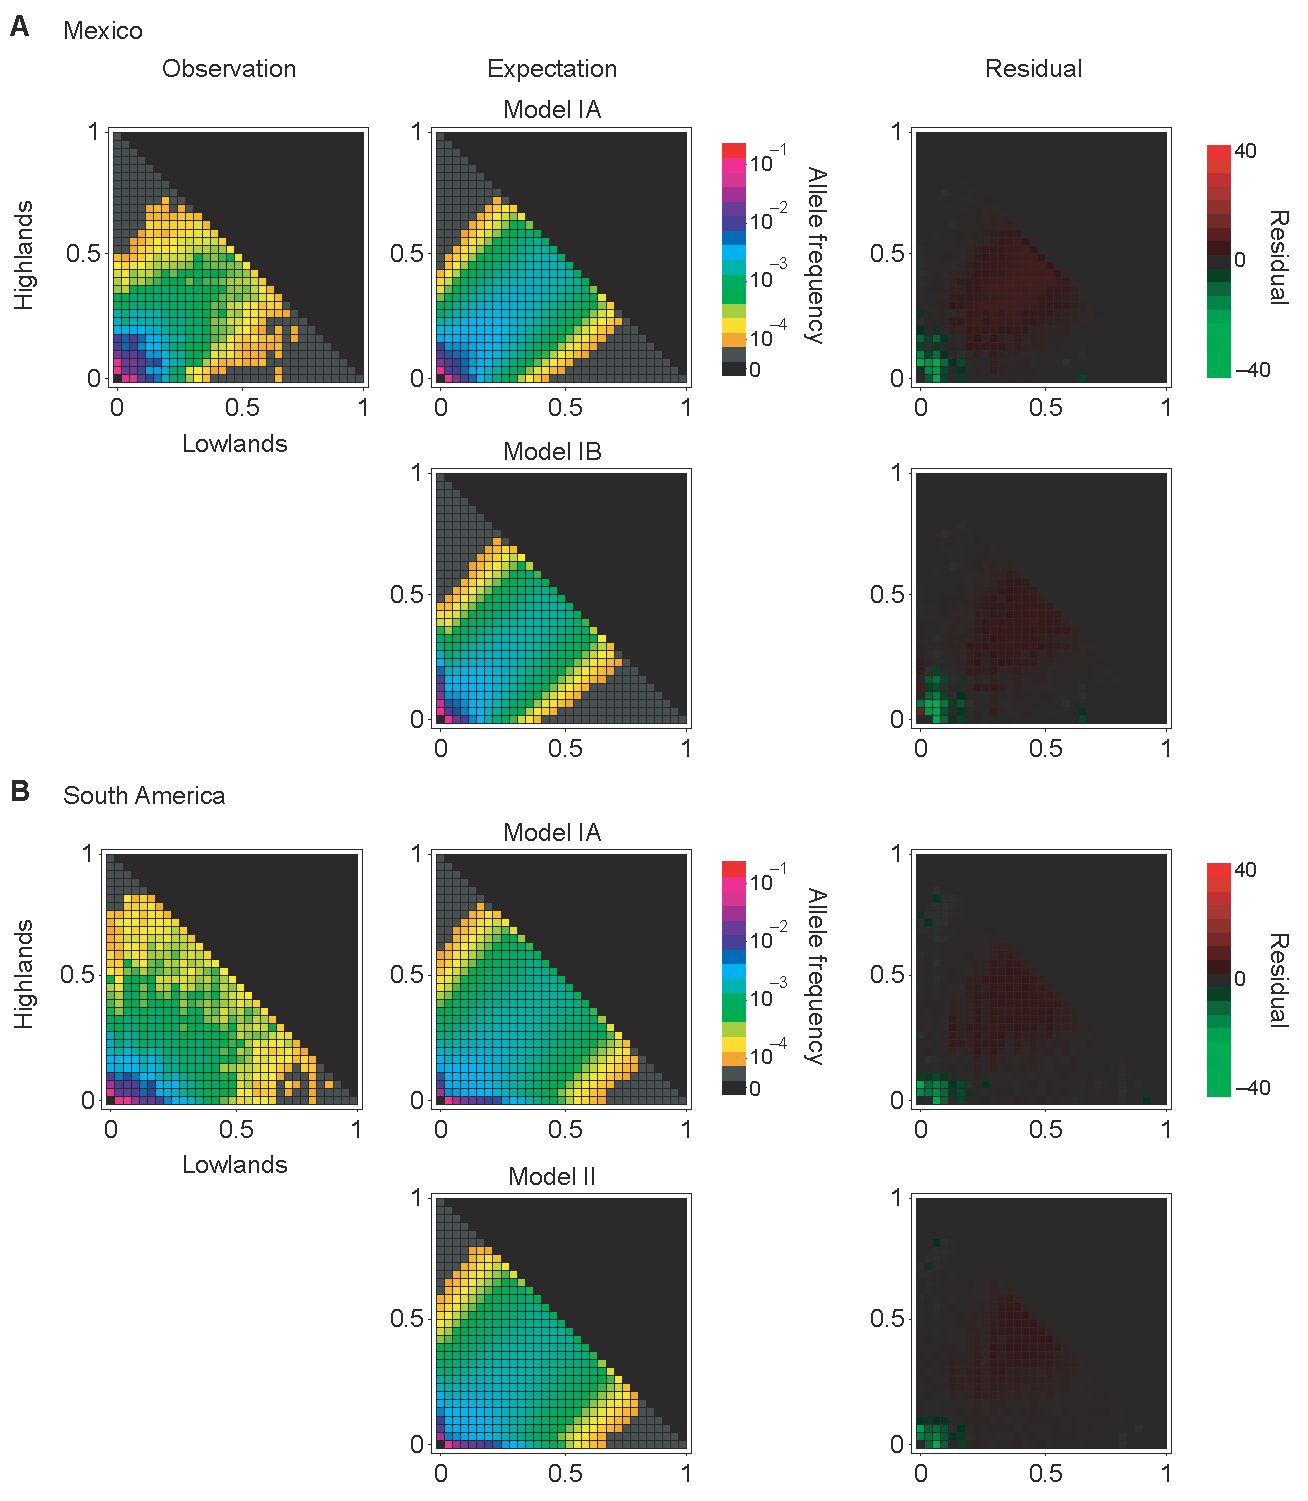
\includegraphics[width=0.5\textwidth]{fig/Fig4}
   \renewcommand{\baselinestretch}{0.9}
   \vspace{-3mm}
   \caption{Observed and expected joint distributions of minor allele frequencies in low- and highland populations in (A) Mexico and (B) S. America. Residuals are calculated as  $(\mbox{model}-\mbox{data})/\sqrt[]{\mbox{model}}$}
\vspace{-6mm}
    \label{JFD}
  \end{center}
\end{figure}
%%%%%%%%%%%%%%%%%%%%%%%%%%%%%%%%%%%%%%%%%% FIGURE


%%%%%%%%%%%%%%%%%%%%%%%%%%%%%%%%%%%%%%%%%% FIGURE
\begin{figure}[tb]   
  \begin{center}
   \vspace{-0mm}
   %\includegraphics[width=0.23\textwidth]{figs/model}
   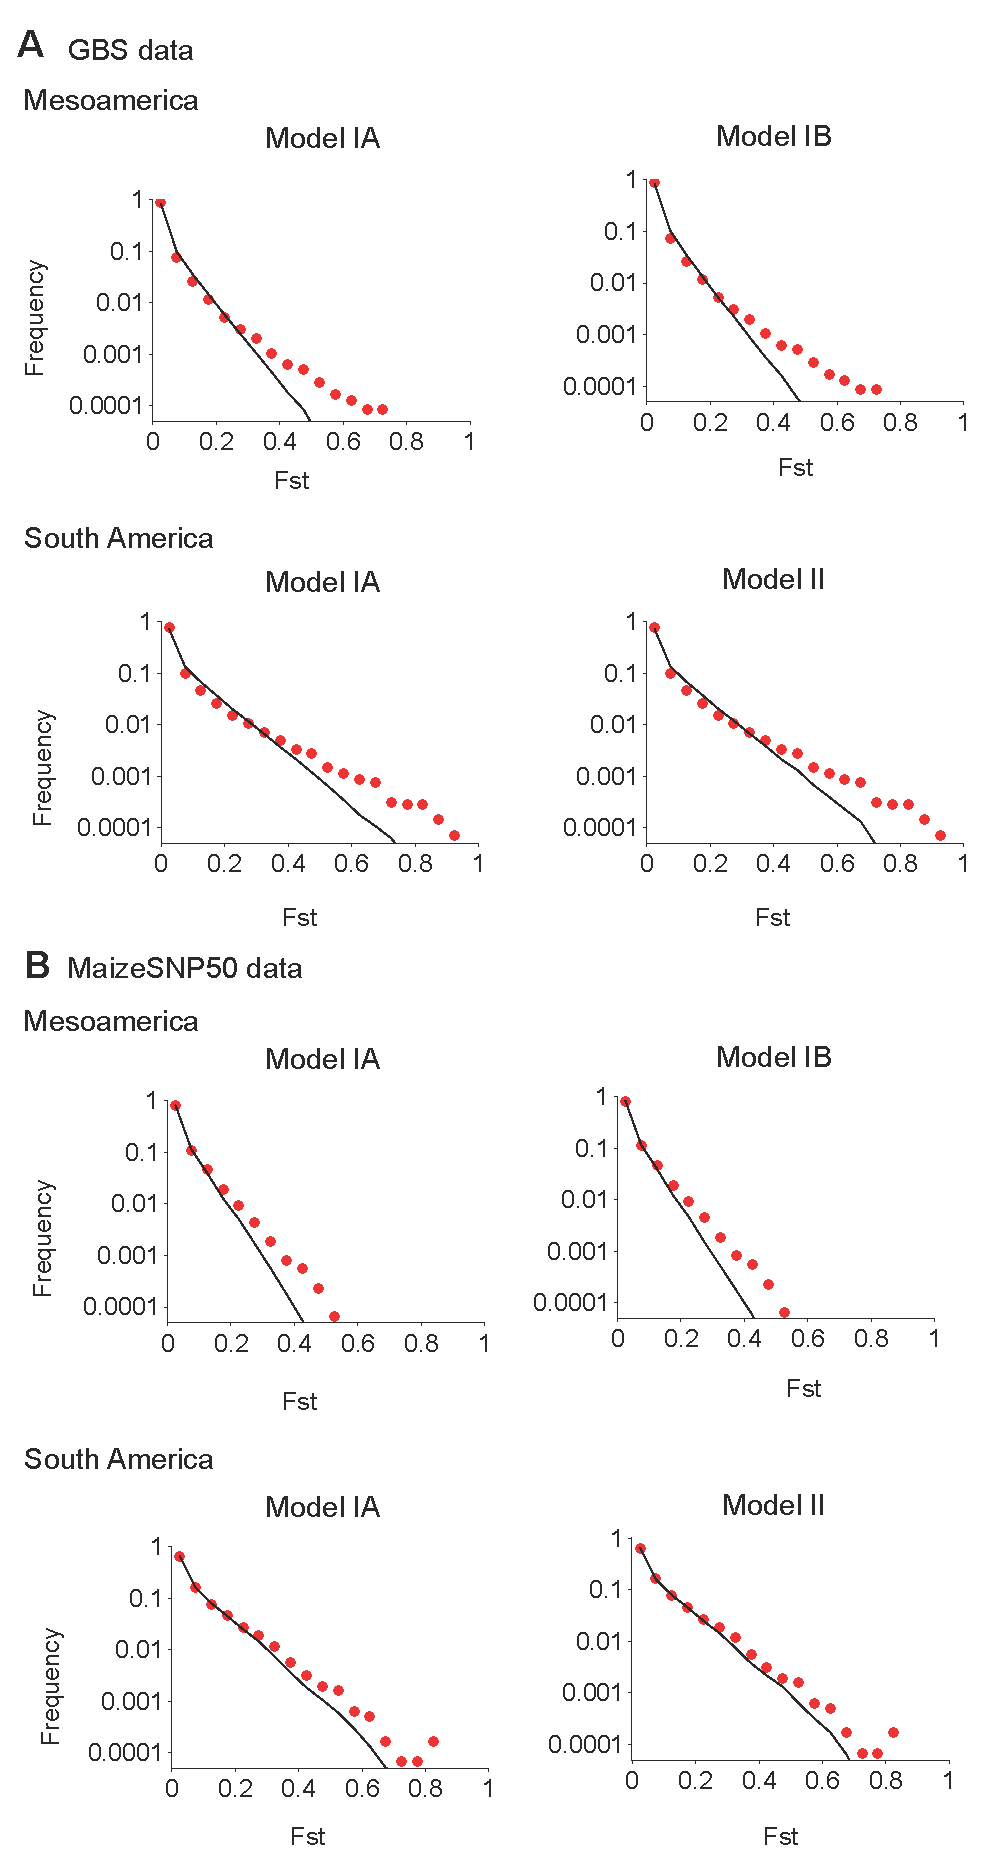
\includegraphics[width=0.45\textwidth]{fig/Fig5}
   \renewcommand{\baselinestretch}{0.9}
   \vspace{-3mm}
   \caption{Observed and expected distributions of $F_{ST}$ values in GBS (A) and MaizeSNP50 data (B).  The \emph{x}-axes represent $F_{ST}$ values.  The \emph{y}-axes represent the frequency of SNPs with $F_{ST}$ values within a bin of 0.05 size.  Red dots and solid lines indicate observed and expected distributions. 
   }
\vspace{-6mm}
    \label{FstDist}
  \end{center}
\end{figure}
%%%%%%%%%%%%%%%%%%%%%%%%%%%%%%%%%%%%%%%%%% FIGURE

\subsection*{Population differentiation under inferred demography}

To provide a null expectation for allele frequency differentiation, we used the joint site frequency distribution (JFD) of lowland and highland populations to estimate parameters of two demographic models  using the maximum likelihood method implemented in $\delta a \delta i$ \cite[]{Gutenkunst_2009_19851460}.  
All models incorporate a domestication bottleneck \cite[]{Wright_2005_15919994} and population differentiation between lowland and highland populations, but differ in their consideration of admixture and ascertainment bias (Figure~\ref{model}; see Materials and Methods for details).

Estimated parameter values are listed in Table~\ref{param}; while the observed and expected JFDs were quite similar for both models,  residuals indicated an excess of rare variants in the observed JFDs in all cases (Figure~\ref{JFD}). 
Under both models IA and IB,  we found expansion in the highland population in Mexico to be unlikely, but a strong bottleneck followed by population expansion is supported in S. American maize in both models IA and II.  
The likelihood value of model IB was higher than the likelihood of model IA by 850 units of log-likelihood (Table~\ref{param}), consistent with analyses suggesting that introgression from \textit{mexicana} played a significant role during the spread of maize into the Mexican highlands \cite[]{Profford_2013}. 

In addition to the parameters listed in Figure~\ref{model}, we investigated the impact of varying the domestication bottleneck size ($N_B$).  
Surprisingly, $N_B$ was estimated to be equal to $N_C$, the population size at the end of the bottleneck, and the likelihood of $N_B<N_C$ was much smaller than for alternative parameterizations (Table~\ref{param},~\ref{supp:param}). This result appears to contradict earlier work using sequences from coding regions to infer a maize domestication bottleneck \cite[]{Eyre-Walker_1998_9539756,Tenaillon_2004_15014173,Wright_2005_15919994}.  
Consistent with \citet{Hufford_2012_22660546}, our genome-wide SNP data show an excess of rare variants relative to expectations under \cite{Wright_2005_15919994}'s bottleneck model (Figure~\ref{JFD}), suggesting a domestication model involving a weaker bottleneck or more rapid population growth.

Comparisons of our empirical $F_{ST}$ values to the null expectation simulated under our demographic models allowed us to identify significantly differentiated SNPs between low- and highland populations. In all cases, observed $F_{ST}$ values were quite similar to those generated under our null models (Figure~\ref{FstDist}), and model choice -- including the parameterization of the domestication bottleneck -- had little impact on the distribution of estimated p-values (Figure~\ref{fig:qq}). 
Thus, hereafter, we show the results under Model IB for Mexican populations and Model II for S. American populations.
We chose $P<0.01$ as an arbitrary cut-off for significant differentiation between low- and highland populations, and identified 687 SNPs in Mexico (687/76,989=0.89\%) and 409 SNPs in South America (409/63,160=0.65\%) as outliers (Figure~\ref{PvDist}).


%%%%%%%%%%%%%%%%%%%%%%%%%%%%%%%%%%%%%%%%%% FIGURE
\begin{figure}[tb]   
  \begin{center}
   \vspace{-0mm}
   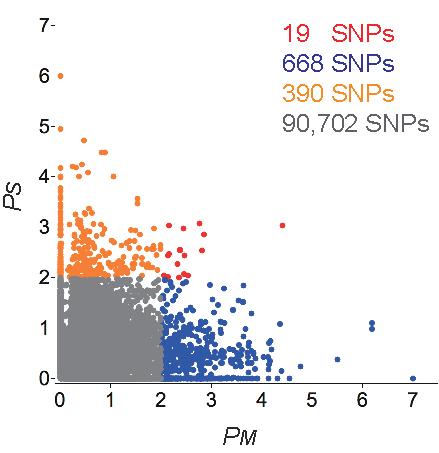
\includegraphics[width=0.4\textwidth]{fig/Fig6}
   \renewcommand{\baselinestretch}{0.9}
   \vspace{-3mm}
   \caption{Scatter plot of $-\log_10 P$-values of observed $F_{ST}$ values based on simulation from estimated demographic models. $P$-values are shown for each SNP in both Mexico (Model IB; $P_M$ on $x$-axis) and South America (Model II; $P_S$ on $y$-axis).  
   Red, blue, orange and gray dots represents SNPs showing significance in both Mexico and South America, only in Mexico, only in South America, respectively (see text for details).
   The number of SNPs in each category is shown in the same color as the points.} 
\vspace{-6mm}
    \label{PvDist}
  \end{center}
\end{figure}
%%%%%%%%%%%%%%%%%%%%%%%%%%%%%%%%%%%%%%%%%% FIGURE
%
%do we know what that clear outlier red SNP is? anything interesting?

\subsection*{Patterns of adaptation}

\subsubsection{Highland versus lowland adaptation}  

Given the historical spread of maize from an origin in the lowlands, it is tempting to assume that significant population differentiation should be primarily due to an increase in frequency of adaptive alleles in the highlands.
To test this hypothesis, we sought to identify the adaptive allele at each locus using comparisons between Mexico and S. America as well as to \emph{parviglumis} (See Supplementary Text  for details).  
Consistent with predictions, we infer that differentiation at 72.3\% (264) and 76.7\% (230) of SNPs in Mexico and S. America is due to adaptation in the highlands after excluding the SNPs with ambiguous patterns (probably due to recombination). 
The majority of these SNPs show patterns of haplotype variation (by PHS test) consistent with our inference (Supplementary Text and Table~\ref{supp:phs}).


\subsubsection{Adaptation via mutation versus standing variation}

In order to characterize patterns of adaptation, we first determined whether SNPs showing high differentiation between the lowlands and the highlands arose primarily through new mutations or standing genetic variation.  
We found that these putatively adaptive variants in both Mexico and South America tended to segregate in Mexican lowland population more often than other SNPs (85.3\% vs. 74.8\% in Mexico, Fisher's exact test (FET) {$P < 10^{-9}$ and 94.8\% vs 87.4\% in South America,  $P< 10^{-4}$).  

%\plr{``segregate in'' -- are these percentages of SNPs that are polymorphic (as opposed to fixed for either allele) in the relevant population?}
%\st{yes. No fixed allele between Mexico and S. America}
%\plr{I don't think I understand.  I'd expect SNPs with high frequency differences between high and lowland to have different chances of polymorphism in lowland populations, somehow.  Why is this meaningful?}
%\jri{agree with peter here. high fst SNPs will have higher mean freq. in maize (avg. between highland and lowland). higher mean freq == older, more likely to be found polymorphic in teosinte. perhaps we should either drop this or reassess taking into account allele freq? same is true for lowland comparison: under neutrality higher freq in highland -> higher freq in lowland and higher fst.}
%\st{In the new ver., P-values are calculated, taking mean freq into account.  So, is it ok?}

We extended this analysis to standing variation in \emph{parviglumis} by retrieving SNP data from 14 \emph{parviglumis} inbred lines included in the Hapmap v2 data set, using only SNPs with $n\geq10$ \cite[]{Chia_2012_22660545,Hufford_2012_22660546}.  
Again we found that putatively adaptive variants were more likely to be polymorphic in \emph{parviglumis} (78.3\% vs. 72.2\% in Mexico, FET {$P < 0.01$ and 80.2\% vs 72.8\% in South America,  $P< 0.01$).  
These results suggest that maize adaptation to high altitude has largely made use of standing genetic variation. 
Recent empirical examples of adaptation from standing variation \cite[Reviewed in ][]{Barrett_2008_18006185,Messer_2013_24075201} and detection of soft selective sweeps in Drosophila \cite[]{Garud_2013_ArXiv} and humans \cite[]{Turchin_2012_22902787,Peter_2012_23071458} suggest this may be a common form of adaptation.
%In the case of maize, lowland-highland divergence events occurred very recently \cite[]{Piperno_2006_69,Perry_2006_16511492,Grobman_2012_22307642} and it would be unlikely that adaptation via \emph{de novo} mutations frequently occurred due to the waiting time required for new beneficial mutations to arise. \jri{tempted to drop this sentence as it seems to preempt our own analytical result? thoughts?}
%Theory also predicts adaptation from standing variation based on estimates of the demography of maize.
Selection from standing variation should be common when the scaled mutation rate (the product of the effective population size, mutation rate and target size), $\Theta\geq1$, as long as the scaled selection coefficient (product of the effective population size and selection coefficient) $Ns$ is large enough \cite[]{Hermisson_2005_15716498}.
Estimates of $\theta$ from synonymous nucleotide diversity in maize ($\cong0.014$ \cite[\emph{e.g.,} ][]{Tenaillon_2004_15014173,Wright_2005_15919994,Ross-Ibarra_2009_19153259}) then suggest adaptation from standing genetic variation would be likely for target sizes larger than a few hundred nucleotides.

%%%%%%%%%%%%%%%%%%%%%%%%%%%%%%%%%%%%%%%%%%%%%%%%%%%%%%%%%%%%
\renewcommand{\arraystretch}{1.1}
\begin{table}[tb]

\begin{center}
 \caption[]{Tanja's $F_{CT}$ between \emph{parviglumis} and \emph{mexicana}\hspace*{0.3cm}}
  \textbf{}\\[-2mm]
{\fontsize{7}{11}\sf
    \begin{tabular}{lcccccccl} 
    \hline
       & & \\[-3mm]
Mexico     & \multicolumn{3}{c}{Number of SNPs}  \\
                                  & Significant & NS          & Proportion  \\
Significant $F_{CT}$ & 25              &   337       & 0.077\\ 
NS                             & 299            &  18,493   & 0.018\\
      \hline
    & & \\[-3mm]
South America     & \multicolumn{3}{c}{Number of SNPs} \\
                                     & Significant & NS           & Proportion  \\
Significant $F_{CT}$    & 10              &   327        & 0.070\\ 
NS                                & 133            &  17,518    & 0.018\\[1mm]
    \hline
  %\multicolumn{4}{l}{$^{a}$ \textcolor{red}{Maybe we should use the number of genetic unit.}}\\
  % \multicolumn{4}{l}{$^{a}$ \textcolor{red}{Sum of the number of SNPs != 91,779 because I excluded SNPs exhibiting}}\\[-0.5mm]
  % \multicolumn{4}{l}{ \textcolor{red}{     monomorphic in Mexico or in South America.}}\\
    \end{tabular}
    \label{tanja}  % caption is needed to make this work
}
\end{center}
\end{table}
\renewcommand{\arraystretch}{1}
%%%%%%%%%%%%%%%%%%%%%%%%%%%%%%%%%%%%%%%%%%%%%%%%%%%%%%%%%%%%



\subsubsection{Adaptation through introgression}

A marked difference between highland adaptation of maize in Mexico and S. America is the potential for adaptation through introgression from wild relatives.  
While maize in Mexico grows in sympatry with both the lowland taxon \textit{parviglumis} and the highland taxon \textit{mexicana}, maize in South America is outside the range of wild \textit{Zea} species.
\citet{Pyhajarvi2013} recently assessed the potential for local adaptation in \textit{parviglumis} and \textit{mexicana} populations, characterizing differentiation between these subspecies using an $F_{ST}$-outlier approach.
We observed a significant excess of overlap between our putatively adaptive SNPs in Mexican maize and those identified in the \citet{Pyhajarvi2013} analysis (Table~\ref{tanja}; $P<10^{-8}$ by FET). 
Similar to that investigation, we found that SNPs with significant $F_{ST}$ $P$-values were enriched in intergenic regions rather than protein coding regions (60.0\% vs. 47.9\%, FET $P < 10^{-7}$ for Mexico; 62.0\% vs. 47.8\%, FET $P<10^{-5}$ for S. America). 
Significant overlap was also observed between S. America and teosinte (Table~\ref{tanja}; $P<10^{-3}$), but the proportion of SNPs was lower than in Mexico.
These data suggest that adaptations in Mexican maize may have been obtained through gene flow with wild relatives.  To more fully explore this hypothesis we evaluated our data in light of introgression identified by \citet{Profford_2013} from \textit{mexicana} into maize in the Mexican highlands.  
The proportion of significant SNPs in introgressed regions in Mexico is significantly higher than found in S. America (FET $P<10^{-6}$).
Outside introgressed regions, the Mexican and S. American populations did not show marked differences in the proportion of significant SNPs (Fisher's exact test, $P=0.036$). These results combined with those from \citet{Profford_2013} suggest that SNPs in introgressed regions have indeed been under selection.  \jri{add sho's rsults about fst in and out of introgressed region}
%\jri{can we say this? if we assume gene flow is correct, wouldn't we expect neutral introgressions from mexicana to show high Fst with lowland maize? maybe delete these sentences and just point out that Tanja's outliers were enriched in matt's regions (i think that's right?)}
%\st{I checked this.  First, I excluded SNPs with significant Fst P-values.  Next, I calculated average Fst within and outside the introgressed regions. The average Fst value within the introgressed regions is 0.032 and that outside those regions is 0.020, so it's ok.}

%When focusing on GUs, we identified 99/586 (14.5\%) and 22/466 (4.7\%) GUs of Mexico- and SA-specific significance in introgressed regions (Fisher's exact test, $P<10^{-6}$). 
%Would the genetic unit numbers work in the tanja table? i liek those numbers and think we should keep if possible.
% ST: the number of overlapped SNPs is not big between Tanja's and mine, so it's hard to check GUs.


\subsubsection{Genetic basis of convergent evolution}

% ST: recombination stuff is moved to subsection "no evidence of parallel adaptation"
%Because linkage disequilibrium in maize decays rapidly \cite[]{Remington_2001_11562485,Tenaillon_2001_11470895} as in our data (Figure~S7), it is plausible that a number of hard sweeps -- strong selection on new mutations -- would be missed by our data, but several lines of evidence suggest to us that this is unlikely.  

While maize adaptation in Mexico and S. America are likely distinguished by unique histories of gene flow with wild relatives, convergent phenotypic evolution in these population may nonetheless have a shared genetic basis.   
Convergent evolution at the nucleotide level should be reflected in an excess of SNPs showing significant differentiation between low- and highland populations in both Mexico and S. America. 
We indeed see such an excess, with 19 SNPs showing $F_{ST}$ \emph{P}-values  $<0.01$ in both Mexico ($P_M$) and S. America ($P_S$), compared to $\approx 5$ expected ($48,370\times 0.01 \times 0.01 \approx 4.8$; $\chi^2$-test, $P\ll0.001$).

%\st{
%DELETE this part.  This q-value approach doesn't work in the new dataset.
%Furthermore, the distribution of $P_M$ in the 712 SNPs with $P_S<0.01$ was highly skewed toward zero, and a similar tendency was observed in $P_S$ in the 935 SNPs with $P_M<0.01$ (Figure~\ref{pval_freq_comparison}).  
%We converted the $P$-values in one population given $P<0.01$ in the other population into $q$-values, and at a false discovery rate of 0.2 we found 117 SNPs with $P_M<0.01 \cap P_S < 0.0169$ or $P_M<0.0247 \cap P_S < 0.01$.   
%We consider these latter SNPS our candidate shared adaptive variants.}

For 13 of 19 SNPs showing putative evidence of shared selection we also had data from \textit{parviglumis} and were able to infer based on patterns of segregation whether these SNPs were potentially adaptive under lowland or highland conditions (Supplemental Text).  
Surprisingly, SNPs identified as shared adaptive variants more frequently showed segregation patterns consistent with lowland  (10 SNPs) rather than highland adaptation (2 SNPs). (1 SNP with an ambiguous pattern). 

%\st{DELETE While the number of shared SNPs is in excess of expectations, we the majority of significant SNPs were significant only in one population (959 $P_M<0.01 \cap P_S > 0.0169$ and 664 $P_S<0.01 \cap P_M>0.0247$; Figure \ref{PvDist}).  }

Our demographic models are not perfect; the observed proportion of rare variants was much higher than expected (Figure~\ref{JFD}).
Nevertheless, this faultiness does not affect our conclusion.
We performed a demographic model-free approach.
We simply defined adaptive variants that showed the top 1\% highest Fst values given $p\pm 0.05$, where $p$ is the mean allele frequency in the highlands and lowlands.
We detected no shared adaptive variant between Mexican and S. American populations by this approach.
\mbh{previous paragraph seems out-of-place and somewhat unnecessary}

In addition to evaluating convergent evolution at the SNP level, we investigated how often different SNPs in the same gene may have been targeted by selection. 
To search for this pattern, we defined a ``genetic unit" or GU as all SNPs within 10kb of a transcript.  
SNPs in an miRNA or second transcript within 10kb of the transcript of interest were excluded.  
We classified SNPs showing significance in Mexico, S. America or in both regions into 778 GUs. 
Of these, 14 GUs contained at least one SNP with a pattern of differentiation suggesting convergent evolution and 2 GUs contained both Mexico-specific and SA-specific significant SNPs. 
Overall, fewer GUs showed evidence of convergent evolution than expected by chance (permutation test; $P<10^{-5}$), with 485 and 277 GUs showing Mexico-specific and SA-specific significant SNPs, respectively.  
Despite similar phenotypes and environments, we thus see little evidence for convergent evolution at either the SNP or the gene (GU) level.  

\jri{this paragraph needs reworking and to jive with the below from peter}
The rarity of convergent evolution in maize contrasts with data from humans \citep{Tennessen_2011_21698142} showing selection on the same genes in multiple pairs of tropical and temperate populations.  
However, in both maize and humans the majority of adaptive variants appear to have been derived from standing variation \cite[]{Tennessen_2011_21698142}.
One difference between these two species is effective population size: the effective population size of maize ($\sim10^5$) is an order of magnitude larger than that in humans \cite[]{Takahata_1997_9114074}.
Humans would therefore have less standing variation as a source of adaptation, perhaps resulting in the same variants being selected in multiple subpopulations (as long as $s$ is sufficiently large and initial frequency is, for example, $>0.1$).
In contrast, maize could maintain a larger number of adaptive variants in the ancestral lowland population.
In this case, if genetic variants produce similar phenotypic effects, they may be selected to high frequency in independent highland regions at random.
Or if Mexican and S. American highlands have slightly different climates, it is feasible that different variants are selected.
The target size of mutations can also increase the variants for adaptation, but there are currently no data regarding mutational target size in maize versus humans.
\plr{You are discussing adaptation from standing variation; what about from new mutation?  This wouldn't require postulating lots of equivalent variants?} \mbh{Sho's data seem to suggest predominance of adaptation from standing variation.  But, given that maize populations are larger than human populations, new mutations would also be more common in maize, which would, I think, lead to less convergence in maize than humans}
In fact, adaptation from multiple standing variants that produce similar phenotypes has previously been observed in maize: the \emph{grassy tillers1} (\emph{gt1}) gene \cite[]{Wills_2013_23825971} contains two artificially selected mutations that reduce ear number.
These mutations both segregate at low frequency in \emph{parviglumis} but have been individually selected to high frequency in different populations of maize.

% ST: LD result is necessary?  Can we say "LD decay looks nice, so genotyping would be nice"?
%Because linkage disequilibrium in maize decays rapidly \cite[]{Remington_2001_11562485,Tenaillon_2001_11470895} as in our data (Figure~S5), it is plausible that a number of hard sweeps -- strong selection on new mutations -- would be missed by our data, but several lines of evidence suggest to us that this is unlikely.  
% MBH:  Not sure where this fits right now...adaptation from standing variation or parallel adaptation...applies to both so maybe a point of discussion at the end?

%Points for discussion (add/delete etc.)
%genomic architecture differences? local adaptation uses regulary in teo (cite Tanja)? But what about Fraser (finds same in humans)
% More likely: target size

%this needs to be moved
%CUTME
%While some have hypothesized that pre-adapted highland maize was transported through Central America to the Andes based on analysis of the \emph{Adh2} locus \citep{Freitas_2003_68}, analysis of larger sets of molecular markers suggests \emph{de novo} highland adaptation in South America \citep{Vigouroux_2008_21632329,vanHeerwaarden_2011_21189301}.  Our result of rare parallel adaptation may be consistent with independent origins of highland populations, not gene flow between the two highland populations.
%MBH:Like the discussion above...any way we could include this somewhere?
% ST:  vote in deleting

%JRI STOPPED HERE

\subsection*{Comparison to theory}

% # \mutrate computation:
% A <- 500; rho <- 5000; sb <- 10^(-(1:4)); xisq <- 30
% sapply( 10^c(-5,-8), function (mu) mu * (2 * rho * A * sb)/xisq )

For a final point of comparison, we assessed the degree of convergence expected under a spatially explicit population genetic model.
We estimated the (maize) population density $\rho$ of the highlands to be around (0.5 people/km$^2$) $\times$ (0.5 ha field/person) $\times$ ($2\times10^4$ plants per field ha) $=$ 5,000 plants per km$^2$.
The area of the Andean highlands is around $A=500\text{km}^2$, leading to a total population of $A \rho = 2.5 \times 10^6$.
%MBH: This seems like a pretty low planting density
%This should be 14K plants per acre, or ~30-35K per hectare. Good catch Matt!!
%  Moved this up here.  I'm not sure what that 14,000 number was doing in the previous draft.  But, added details behind this calculation.  Should I change anything?
%  Note that 0.5 people/km2 is close to the other number we came up with of "one village per 15km" (which gets 0.4444 people/km2).
% I think these numbers are OK.  It's ~8000 plants per acre, which is really low, but we're talking prehistoric times.  In the 1960's they were still experimenting with 9-18000 per acres (http://trace.tennessee.edu/cgi/viewcontent.cgi?article=1321&context=utk_agbulletin) in Tennessee!
Combined with an offspring variance of $\xi^2 = 30$, we can compute the rate, $\mutrate$, at which newly adapted alleles arise in the population.
We observe that even if there is strong selection for an allele at high elevation ($s_b=0.1$), a single-base mutation with mutation rate $\mu=10^{-8}$ would still take at least 6,000 generations to appear and fix.
On the other hand, a kilobase-sized target with mutation rate $\mu=10^{-5}$ with this selection coefficient would appear and begin to fix in only 6 generations, while more weakly selected alleles with $s_b$ of $10^{-2}$ or $10^{-3}$ would take hundreds or thousands of generations, respectively.
(Note that the time scales linearly with the selection coefficient: at these values $\Tmut = 1/\mutrate \approx \mu s_b \times 1.6\times 10^5$.)
Therefore, we might expect to see convergent changes of similar effect at the level of genes (e.g.\ disabling mutations), but would not expect to see adaptive SNPs that arise through independent mutation in the two populations.

% # Tmig computation:
% A <- 500; rho <- 5000; sm <- 10^(-(1:4)); xisq <- 30; sigma <- 1.8
% 1/(sqrt(2*sm)/sigma)
% sapply( 1000*(1:4), function (R) 1 / ( A * rho * ( sqrt(2*sm) / xisq ) * exp(- sqrt(2*sm)*R/sigma ) ) )
% Ne <- (561/10^5)*A*rho 
% Ne  # = 14025
% sapply( 1000*(1:4), function (R) 1 / ( Ne * exp(- sqrt(2*sm)*R/sigma ) ) )

While convergent SNP changes seem unlikely from new mutation, the potential remains for gene flow between highland regions.
From the demographic model above we have estimated that $\sigma \approx 1.8$ kilometers per generation, so with $10^{-1} \ge s_m \ge 10^{-4}$ the distance $\sigma/\sqrt{2s_m}$ over which the frequency of a highland-adaptive, lowland-deleterious allele decays into the lowlands is still short: between 4 and 150 kilometers.
Since the Mexican and Andean highlands are around 4,000 km apart, the time needed for a rare allele, with selective cost $s_m=10^{-3}$ in the lowlands, to transit between the two highland regions is $\Tmig \approx 5 \times 10^{34}$ generations.
In other words, from these calculations it is almost impossible that an allele that is deleterious at low elevation with $s_m=10^{-3}$ would ever transit from the Mexican to the Andean highlands.
If the selection against the allele is even weaker ($s_m=10^{-4}$) it is still expected to take $\Tmig = 1.8 \times 10^8$ generations.
However, shorter distances could be transited by very weakly deleterious alleles -- if the distance between highland patches $R$ is 1,000 km (or if $\sigma$ is four times larger) then with $s_m=10^{-4}$ the time $\Tmig$ is about 1.6 generations -- so, adaptation by migration is certain in the known timeframe of maize diffusion.
This is strongly dependent on the magnitude of the deleterious selection coefficient: for example, with $s_m=10^{-3}$, $\Tmig$ is $2.3 \times 10^6$ generations.

Our analysis suggests that even when highland-adaptive mutations are weakly deleterious in the lowlands, gene flow will not result in shared adaptations.
The situation where these are neutral in the lowlands is more difficult to model, but we can make some informed guesses.
For maize in the Andean highlands to have inherited a highland-adapted allele from the Mexican highlands, those Andean plants must be directly descended from highland Mexican plants that lived more recently than the appearance of the adaptive allele.
In other words, the ancestral lineages along which the modern Andean plants have inherited at that locus must trace back to the Mexican highlands.
If the allele is neutral in the lowlands, we can treat the movement of these lineages as a neutral process, using the framework of coalescent theory \citep{wakeley2005coalescent}.
To do this, we need to follow \emph{all} of the $N \approx 2.5 \times 10^6$ lineages backwards; these quickly coalesce to fewer $m$ lineages in approximately $\sum_{k=m}^N \frac{2N}{\xi^2 k(k+1)} \approx 1.25 \times 10^5/m$ generations, leaving about 1000 lineages after 100 generations that are spread over a larger area.
The displacement of a lineage after $m$ generations has variance $m \sigma^2$ and is approximately Gaussian.
If we assume that $n$ lineages are independent, and $Z_n$ is the distance to the furthest lineage, then $\P\{ Z_n / \sqrt{m \sigma^2} \le x /\sqrt{2 \log n} + \sqrt{2 \log n} - (1/2) (\log \log n + \log 4 \pi)/\sqrt{2 \log n} \} \approx \exp( - e^{-x} )$ \citep{berman1964limit}.
With $n=1000$, the typical distance to the furthest displacement after $m=1000$ generations is $\sqrt{2 \sigma^2 m \log n} \approx 212$km; after $m=6000$ generations it is $\approx 518$km.
In either case, the chance that the maximum is larger than 1,000km after 6,000 generations is well less than $10^{-4}$.
Of course, this is under an equilibrium population model; and maize reached the Andean highlands only around 4,000 years ago.
Nonetheless, this suggests that even highland-adapted alleles that are merely neutral in the lowlands would have difficulty moving between the Mexican and Andean highlands in a few thousand generations.

Based on our spatially explicit population genetic model, convergent evolution involving identical nucleotide changes is quite unlikely under either scenarios of independent mutation or transit of Central America by undirected (diffusive) sharing of seed. 
However, independent mutations could be expected in kilobase-sized targets \mbh{I'm a little confused about what is meant by a kilobase-sized target...would this mean that mutation at every nucleotide over this distance produced the same phenotypic effect?  This wouldn't be possible.}, suggesting there might be signal for genes that share adaptive changes.
These conclusions could change if we drastically underestimated the rate of very-long-distance sharing of seed, e.g.\ if sharing across hundreds of kilometers was common at some point.

